\documentclass[1p]{elsarticle_modified}
%\bibliographystyle{elsarticle-num}

%\usepackage[colorlinks]{hyperref}
%\usepackage{abbrmath_seonhwa} %\Abb, \Ascr, \Acal ,\Abf, \Afrak
\usepackage{amsfonts}
\usepackage{amssymb}
\usepackage{amsmath}
\usepackage{amsthm}
\usepackage{scalefnt}
\usepackage{amsbsy}
\usepackage{kotex}
\usepackage{caption}
\usepackage{subfig}
\usepackage{color}
\usepackage{graphicx}
\usepackage{xcolor} %% white, black, red, green, blue, cyan, magenta, yellow
\usepackage{float}
\usepackage{setspace}
\usepackage{hyperref}

\usepackage{tikz}
\usetikzlibrary{arrows}

\usepackage{multirow}
\usepackage{array} % fixed length table
\usepackage{hhline}

%%%%%%%%%%%%%%%%%%%%%
\makeatletter
\renewcommand*\env@matrix[1][\arraystretch]{%
	\edef\arraystretch{#1}%
	\hskip -\arraycolsep
	\let\@ifnextchar\new@ifnextchar
	\array{*\c@MaxMatrixCols c}}
\makeatother %https://tex.stackexchange.com/questions/14071/how-can-i-increase-the-line-spacing-in-a-matrix
%%%%%%%%%%%%%%%

\usepackage[normalem]{ulem}

\newcommand{\msout}[1]{\ifmmode\text{\sout{\ensuremath{#1}}}\else\sout{#1}\fi}
%SOURCE: \msout is \stkout macro in https://tex.stackexchange.com/questions/20609/strikeout-in-math-mode

\newcommand{\cancel}[1]{
	\ifmmode
	{\color{red}\msout{#1}}
	\else
	{\color{red}\sout{#1}}
	\fi
}

\newcommand{\add}[1]{
	{\color{blue}\uwave{#1}}
}

\newcommand{\replace}[2]{
	\ifmmode
	{\color{red}\msout{#1}}{\color{blue}\uwave{#2}}
	\else
	{\color{red}\sout{#1}}{\color{blue}\uwave{#2}}
	\fi
}

\newcommand{\Sol}{\mathcal{S}} %segment
\newcommand{\D}{D} %diagram
\newcommand{\A}{\mathcal{A}} %arc


%%%%%%%%%%%%%%%%%%%%%%%%%%%%%5 test

\def\sl{\operatorname{\textup{SL}}(2,\Cbb)}
\def\psl{\operatorname{\textup{PSL}}(2,\Cbb)}
\def\quan{\mkern 1mu \triangleright \mkern 1mu}

\theoremstyle{definition}
\newtheorem{thm}{Theorem}[section]
\newtheorem{prop}[thm]{Proposition}
\newtheorem{lem}[thm]{Lemma}
\newtheorem{ques}[thm]{Question}
\newtheorem{cor}[thm]{Corollary}
\newtheorem{defn}[thm]{Definition}
\newtheorem{exam}[thm]{Example}
\newtheorem{rmk}[thm]{Remark}
\newtheorem{alg}[thm]{Algorithm}

\newcommand{\I}{\sqrt{-1}}
\begin{document}

%\begin{frontmatter}
%
%\title{Boundary parabolic representations of knots up to 8 crossings}
%
%%% Group authors per affiliation:
%\author{Yunhi Cho} 
%\address{Department of Mathematics, University of Seoul, Seoul, Korea}
%\ead{yhcho@uos.ac.kr}
%
%
%\author{Seonhwa Kim} %\fnref{s_kim}}
%\address{Center for Geometry and Physics, Institute for Basic Science, Pohang, 37673, Korea}
%\ead{ryeona17@ibs.re.kr}
%
%\author{Hyuk Kim}
%\address{Department of Mathematical Sciences, Seoul National University, Seoul 08826, Korea}
%\ead{hyukkim@snu.ac.kr}
%
%\author{Seokbeom Yoon}
%\address{Department of Mathematical Sciences, Seoul National University, Seoul, 08826,  Korea}
%\ead{sbyoon15@snu.ac.kr}
%
%\begin{abstract}
%We find all boundary parabolic representation of knots up to 8 crossings.
%
%\end{abstract}
%\begin{keyword}
%    \MSC[2010] 57M25 
%\end{keyword}
%
%\end{frontmatter}

%\linenumbers
%\tableofcontents
%
\newcommand\colored[1]{\textcolor{white}{\rule[-0.35ex]{0.8em}{1.4ex}}\kern-0.8em\color{red} #1}%
%\newcommand\colored[1]{\textcolor{white}{ #1}\kern-2.17ex	\textcolor{white}{ #1}\kern-1.81ex	\textcolor{white}{ #1}\kern-2.15ex\color{red}#1	}

{\Large $\underline{11n_{130}~(K11n_{130})}$}

\setlength{\tabcolsep}{10pt}
\renewcommand{\arraystretch}{1.6}
\vspace{1cm}\begin{tabular}{m{100pt}>{\centering\arraybackslash}m{274pt}}
\multirow{5}{120pt}{
	\centering
	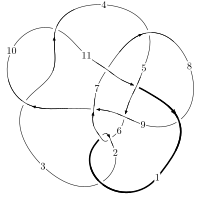
\includegraphics[width=112pt]{../../../GIT/diagram.site/Diagrams/png/746_11n_130.png}\\
\ \ \ A knot diagram\footnotemark}&
\allowdisplaybreaks
\textbf{Linearized knot diagam} \\
\cline{2-2}
 &
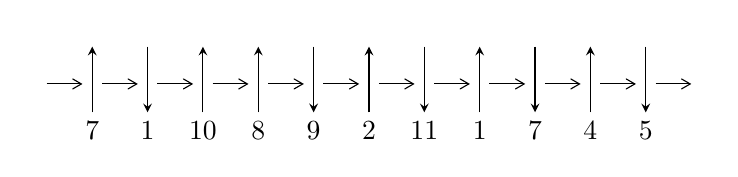
\begin{tikzpicture}[x=20pt, y=17pt]
	% nodes
	\node (C0) at (0, 0) {};
	\node (C1) at (1, 0) {};
	\node (C1U) at (1, +1) {};
	\node (C1D) at (1, -1) {7};

	\node (C2) at (2, 0) {};
	\node (C2U) at (2, +1) {};
	\node (C2D) at (2, -1) {1};

	\node (C3) at (3, 0) {};
	\node (C3U) at (3, +1) {};
	\node (C3D) at (3, -1) {10};

	\node (C4) at (4, 0) {};
	\node (C4U) at (4, +1) {};
	\node (C4D) at (4, -1) {8};

	\node (C5) at (5, 0) {};
	\node (C5U) at (5, +1) {};
	\node (C5D) at (5, -1) {9};

	\node (C6) at (6, 0) {};
	\node (C6U) at (6, +1) {};
	\node (C6D) at (6, -1) {2};

	\node (C7) at (7, 0) {};
	\node (C7U) at (7, +1) {};
	\node (C7D) at (7, -1) {11};

	\node (C8) at (8, 0) {};
	\node (C8U) at (8, +1) {};
	\node (C8D) at (8, -1) {1};

	\node (C9) at (9, 0) {};
	\node (C9U) at (9, +1) {};
	\node (C9D) at (9, -1) {7};

	\node (C10) at (10, 0) {};
	\node (C10U) at (10, +1) {};
	\node (C10D) at (10, -1) {4};

	\node (C11) at (11, 0) {};
	\node (C11U) at (11, +1) {};
	\node (C11D) at (11, -1) {5};
	\node (C12) at (12, 0) {};

	% arrows
	\draw[->,>={angle 60}]
	(C0) edge (C1) (C1) edge (C2) (C2) edge (C3) (C3) edge (C4) (C4) edge (C5) (C5) edge (C6) (C6) edge (C7) (C7) edge (C8) (C8) edge (C9) (C9) edge (C10) (C10) edge (C11) (C11) edge (C12) ;	\draw[->,>=stealth]
	(C1D) edge (C1U) (C2U) edge (C2D) (C3D) edge (C3U) (C4D) edge (C4U) (C5U) edge (C5D) (C6D) edge (C6U) (C7U) edge (C7D) (C8D) edge (C8U) (C9U) edge (C9D) (C10D) edge (C10U) (C11U) edge (C11D) ;
	\end{tikzpicture} \\
\hhline{~~} \\& 
\textbf{Solving Sequence} \\ \cline{2-2} 
 &
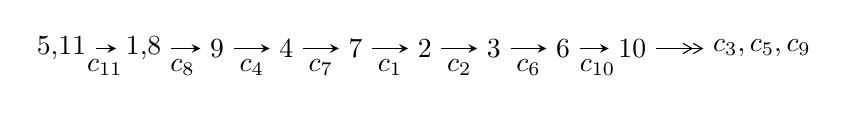
\begin{tikzpicture}[x=25pt, y=7pt]
	% node
	\node (A0) at (-1/8, 0) {5,11};
	\node (A1) at (17/16, 0) {1,8};
	\node (A2) at (17/8, 0) {9};
	\node (A3) at (25/8, 0) {4};
	\node (A4) at (33/8, 0) {7};
	\node (A5) at (41/8, 0) {2};
	\node (A6) at (49/8, 0) {3};
	\node (A7) at (57/8, 0) {6};
	\node (A8) at (65/8, 0) {10};
	\node (C1) at (1/2, -1) {$c_{11}$};
	\node (C2) at (13/8, -1) {$c_{8}$};
	\node (C3) at (21/8, -1) {$c_{4}$};
	\node (C4) at (29/8, -1) {$c_{7}$};
	\node (C5) at (37/8, -1) {$c_{1}$};
	\node (C6) at (45/8, -1) {$c_{2}$};
	\node (C7) at (53/8, -1) {$c_{6}$};
	\node (C8) at (61/8, -1) {$c_{10}$};
	\node (A9) at (10, 0) {$c_{3},c_{5},c_{9}$};

	% edge
	\draw[->,>=stealth]	
	(A0) edge (A1) (A1) edge (A2) (A2) edge (A3) (A3) edge (A4) (A4) edge (A5) (A5) edge (A6) (A6) edge (A7) (A7) edge (A8) ;
	\draw[->>,>={angle 60}]	
	(A8) edge (A9);
\end{tikzpicture} \\ 

\end{tabular} \\

\footnotetext{
The image of knot diagram is generated by the software ``\textbf{Draw programme}" developed by Andrew Bartholomew(\url{http://www.layer8.co.uk/maths/draw/index.htm\#Running-draw}), where we modified some parts for our purpose(\url{https://github.com/CATsTAILs/LinksPainter}).
}\phantom \\ \newline 
\centering \textbf{Ideals for irreducible components\footnotemark of $X_{\text{par}}$} 
 
\begin{align*}
I^u_{1}&=\langle 
-2.64498\times10^{39} u^{36}-5.83142\times10^{39} u^{35}+\cdots+9.36297\times10^{38} b-1.79289\times10^{40},\\
\phantom{I^u_{1}}&\phantom{= \langle  }8.32208\times10^{40} u^{36}+2.24302\times10^{41} u^{35}+\cdots+1.02993\times10^{40} a+1.49267\times10^{42},\;u^{37}+2 u^{36}+\cdots-8 u-11\rangle \\
I^u_{2}&=\langle 
5 u^{10}+19 u^9+8 u^8+9 u^7+20 u^6+86 u^5+142 u^4+71 u^3-71 u^2+67 b+39 u+64,\\
\phantom{I^u_{2}}&\phantom{= \langle  }5 u^{10}-48 u^9+8 u^8+76 u^7-47 u^6-249 u^5+75 u^4+138 u^3-4 u^2+67 a-95 u+131,\\
\phantom{I^u_{2}}&\phantom{= \langle  }u^{11}+u^{10}- u^9+7 u^7+6 u^6- u^5- u^4+5 u^3+2 u^2- u-1\rangle \\
\\
\end{align*}
\raggedright * 2 irreducible components of $\dim_{\mathbb{C}}=0$, with total 48 representations.\\
\footnotetext{All coefficients of polynomials are rational numbers. But the coefficients are sometimes approximated in decimal forms when there is not enough margin.}
\newpage
\renewcommand{\arraystretch}{1}
\centering \section*{I. $I^u_{1}= \langle -2.64\times10^{39} u^{36}-5.83\times10^{39} u^{35}+\cdots+9.36\times10^{38} b-1.79\times10^{40},\;8.32\times10^{40} u^{36}+2.24\times10^{41} u^{35}+\cdots+1.03\times10^{40} a+1.49\times10^{42},\;u^{37}+2 u^{36}+\cdots-8 u-11 \rangle$}
\flushleft \textbf{(i) Arc colorings}\\
\begin{tabular}{m{7pt} m{180pt} m{7pt} m{180pt} }
\flushright $a_{5}=$&$\begin{pmatrix}0\\u\end{pmatrix}$ \\
\flushright $a_{11}=$&$\begin{pmatrix}1\\0\end{pmatrix}$ \\
\flushright $a_{1}=$&$\begin{pmatrix}1\\u^2\end{pmatrix}$ \\
\flushright $a_{8}=$&$\begin{pmatrix}-8.08027 u^{36}-21.7785 u^{35}+\cdots-344.393 u-144.929\\2.82494 u^{36}+6.22818 u^{35}+\cdots+78.1053 u+19.1487\end{pmatrix}$ \\
\flushright $a_{9}=$&$\begin{pmatrix}-1.86142 u^{36}-6.80771 u^{35}+\cdots-132.462 u-63.9835\\5.72773 u^{36}+12.8467 u^{35}+\cdots+166.777 u+47.0123\end{pmatrix}$ \\
\flushright $a_{4}=$&$\begin{pmatrix}-14.5710 u^{36}-35.2438 u^{35}+\cdots-475.357 u-170.402\\-4.84473 u^{36}-12.7993 u^{35}+\cdots-193.507 u-68.6348\end{pmatrix}$ \\
\flushright $a_{7}=$&$\begin{pmatrix}-5.25533 u^{36}-15.5503 u^{35}+\cdots-266.288 u-125.781\\2.82494 u^{36}+6.22818 u^{35}+\cdots+78.1053 u+19.1487\end{pmatrix}$ \\
\flushright $a_{2}=$&$\begin{pmatrix}7.55117 u^{36}+20.4537 u^{35}+\cdots+318.954 u+177.930\\4.57906 u^{36}+12.5897 u^{35}+\cdots+193.139 u+107.947\end{pmatrix}$ \\
\flushright $a_{3}=$&$\begin{pmatrix}7.22065 u^{36}+17.5684 u^{35}+\cdots+251.689 u+128.847\\4.47610 u^{36}+11.7558 u^{35}+\cdots+171.709 u+83.4806\end{pmatrix}$ \\
\flushright $a_{6}=$&$\begin{pmatrix}-9.28201 u^{36}-21.1993 u^{35}+\cdots-266.287 u-108.443\\0.126287 u^{36}+2.51101 u^{35}+\cdots+72.2964 u+34.4863\end{pmatrix}$ \\
\flushright $a_{10}=$&$\begin{pmatrix}2.42894 u^{36}+8.72585 u^{35}+\cdots+164.941 u+113.830\\2.47797 u^{36}+5.69993 u^{35}+\cdots+64.9436 u+35.7552\end{pmatrix}$\\ \flushright $a_{10}=$&$\begin{pmatrix}2.42894 u^{36}+8.72585 u^{35}+\cdots+164.941 u+113.830\\2.47797 u^{36}+5.69993 u^{35}+\cdots+64.9436 u+35.7552\end{pmatrix}$\\&\end{tabular}
\flushleft \textbf{(ii) Obstruction class $= -1$}\\~\\
\flushleft \textbf{(iii) Cusp Shapes $= -28.2238 u^{36}-73.9995 u^{35}+\cdots-1024.01 u-467.975$}\\~\\
\newpage\renewcommand{\arraystretch}{1}
\flushleft \textbf{(iv) u-Polynomials at the component}\newline \\
\begin{tabular}{m{50pt}|m{274pt}}
Crossings & \hspace{64pt}u-Polynomials at each crossing \\
\hline $$\begin{aligned}c_{1},c_{6}\end{aligned}$$&$\begin{aligned}
&u^{37}+24 u^{35}+\cdots-4 u+1
\end{aligned}$\\
\hline $$\begin{aligned}c_{2}\end{aligned}$$&$\begin{aligned}
&u^{37}+48 u^{36}+\cdots+8 u-1
\end{aligned}$\\
\hline $$\begin{aligned}c_{3},c_{10}\end{aligned}$$&$\begin{aligned}
&u^{37}- u^{36}+\cdots+6 u+1
\end{aligned}$\\
\hline $$\begin{aligned}c_{4}\end{aligned}$$&$\begin{aligned}
&u^{37}-3 u^{36}+\cdots+12 u+1
\end{aligned}$\\
\hline $$\begin{aligned}c_{5}\end{aligned}$$&$\begin{aligned}
&u^{37}- u^{36}+\cdots+1746 u+367
\end{aligned}$\\
\hline $$\begin{aligned}c_{7}\end{aligned}$$&$\begin{aligned}
&u^{37}+4 u^{36}+\cdots-8 u+1
\end{aligned}$\\
\hline $$\begin{aligned}c_{8}\end{aligned}$$&$\begin{aligned}
&u^{37}+10 u^{35}+\cdots-75 u+23
\end{aligned}$\\
\hline $$\begin{aligned}c_{9}\end{aligned}$$&$\begin{aligned}
&u^{37}+6 u^{36}+\cdots-6703 u+583
\end{aligned}$\\
\hline $$\begin{aligned}c_{11}\end{aligned}$$&$\begin{aligned}
&u^{37}+2 u^{36}+\cdots-8 u-11
\end{aligned}$\\
\hline
\end{tabular}\\~\\
\newpage\renewcommand{\arraystretch}{1}
\flushleft \textbf{(v) Riley Polynomials at the component}\newline \\
\begin{tabular}{m{50pt}|m{274pt}}
Crossings & \hspace{64pt}Riley Polynomials at each crossing \\
\hline $$\begin{aligned}c_{1},c_{6}\end{aligned}$$&$\begin{aligned}
&y^{37}+48 y^{36}+\cdots+8 y-1
\end{aligned}$\\
\hline $$\begin{aligned}c_{2}\end{aligned}$$&$\begin{aligned}
&y^{37}-112 y^{36}+\cdots-100 y-1
\end{aligned}$\\
\hline $$\begin{aligned}c_{3},c_{10}\end{aligned}$$&$\begin{aligned}
&y^{37}-17 y^{36}+\cdots+22 y-1
\end{aligned}$\\
\hline $$\begin{aligned}c_{4}\end{aligned}$$&$\begin{aligned}
&y^{37}-3 y^{36}+\cdots+24 y-1
\end{aligned}$\\
\hline $$\begin{aligned}c_{5}\end{aligned}$$&$\begin{aligned}
&y^{37}-53 y^{36}+\cdots+2094316 y-134689
\end{aligned}$\\
\hline $$\begin{aligned}c_{7}\end{aligned}$$&$\begin{aligned}
&y^{37}+2 y^{36}+\cdots-56 y^2-1
\end{aligned}$\\
\hline $$\begin{aligned}c_{8}\end{aligned}$$&$\begin{aligned}
&y^{37}+20 y^{36}+\cdots-44975 y-529
\end{aligned}$\\
\hline $$\begin{aligned}c_{9}\end{aligned}$$&$\begin{aligned}
&y^{37}-66 y^{36}+\cdots+4068905 y-339889
\end{aligned}$\\
\hline $$\begin{aligned}c_{11}\end{aligned}$$&$\begin{aligned}
&y^{37}-10 y^{36}+\cdots+2308 y-121
\end{aligned}$\\
\hline
\end{tabular}\\~\\
\newpage\flushleft \textbf{(vi) Complex Volumes and Cusp Shapes}
$$\begin{array}{c|c|c}  
\text{Solutions to }I^u_{1}& \I (\text{vol} + \sqrt{-1}CS) & \text{Cusp shape}\\
 \hline 
\begin{aligned}
u &= -0.601373 + 0.797904 I \\
a &= \phantom{-}0.100319 - 0.818260 I \\
b &= -0.125544 + 0.666416 I\end{aligned}
 & \phantom{-}0.33153 + 1.56965 I & \phantom{-}1.84729 - 2.87829 I \\ \hline\begin{aligned}
u &= -0.601373 - 0.797904 I \\
a &= \phantom{-}0.100319 + 0.818260 I \\
b &= -0.125544 - 0.666416 I\end{aligned}
 & \phantom{-}0.33153 - 1.56965 I & \phantom{-}1.84729 + 2.87829 I \\ \hline\begin{aligned}
u &= -0.756589 + 0.697163 I \\
a &= \phantom{-}0.048994 - 0.966661 I \\
b &= -0.592884 + 1.189630 I\end{aligned}
 & \phantom{-}0.52746 + 2.09006 I & \phantom{-}0.36189 - 3.60216 I \\ \hline\begin{aligned}
u &= -0.756589 - 0.697163 I \\
a &= \phantom{-}0.048994 + 0.966661 I \\
b &= -0.592884 - 1.189630 I\end{aligned}
 & \phantom{-}0.52746 - 2.09006 I & \phantom{-}0.36189 + 3.60216 I \\ \hline\begin{aligned}
u &= \phantom{-}0.746755 + 0.717340 I \\
a &= \phantom{-}0.24852 - 1.52698 I \\
b &= \phantom{-}0.832075 + 0.932954 I\end{aligned}
 & \phantom{-}3.60755 - 4.86664 I & \phantom{-}5.83345 + 5.56346 I \\ \hline\begin{aligned}
u &= \phantom{-}0.746755 - 0.717340 I \\
a &= \phantom{-}0.24852 + 1.52698 I \\
b &= \phantom{-}0.832075 - 0.932954 I\end{aligned}
 & \phantom{-}3.60755 + 4.86664 I & \phantom{-}5.83345 - 5.56346 I \\ \hline\begin{aligned}
u &= -0.850079 + 0.415638 I \\
a &= \phantom{-}0.200244 + 0.592775 I \\
b &= -1.43302 - 1.13498 I\end{aligned}
 & -9.44422 + 4.54412 I & -2.91144 - 6.06217 I \\ \hline\begin{aligned}
u &= -0.850079 - 0.415638 I \\
a &= \phantom{-}0.200244 - 0.592775 I \\
b &= -1.43302 + 1.13498 I\end{aligned}
 & -9.44422 - 4.54412 I & -2.91144 + 6.06217 I \\ \hline\begin{aligned}
u &= \phantom{-}0.833991 + 0.353566 I \\
a &= \phantom{-}0.238282 + 1.378690 I \\
b &= \phantom{-}0.48049 - 1.49168 I\end{aligned}
 & -9.78588 + 0.61235 I & -3.21523 + 0.70893 I \\ \hline\begin{aligned}
u &= \phantom{-}0.833991 - 0.353566 I \\
a &= \phantom{-}0.238282 - 1.378690 I \\
b &= \phantom{-}0.48049 + 1.49168 I\end{aligned}
 & -9.78588 - 0.61235 I & -3.21523 - 0.70893 I\\
 \hline 
 \end{array}$$\newpage$$\begin{array}{c|c|c}  
\text{Solutions to }I^u_{1}& \I (\text{vol} + \sqrt{-1}CS) & \text{Cusp shape}\\
 \hline 
\begin{aligned}
u &= -0.820454 + 0.302238 I \\
a &= \phantom{-}0.649750 - 0.760838 I \\
b &= \phantom{-}0.367432 - 0.280099 I\end{aligned}
 & -0.44492 + 2.47536 I & -1.10953 - 5.85952 I \\ \hline\begin{aligned}
u &= -0.820454 - 0.302238 I \\
a &= \phantom{-}0.649750 + 0.760838 I \\
b &= \phantom{-}0.367432 + 0.280099 I\end{aligned}
 & -0.44492 - 2.47536 I & -1.10953 + 5.85952 I \\ \hline\begin{aligned}
u &= -0.709146 + 0.450731 I \\
a &= -2.09178 - 0.67084 I \\
b &= -1.020550 + 0.314178 I\end{aligned}
 & -8.92085 - 1.02999 I & -3.37249 - 2.08147 I \\ \hline\begin{aligned}
u &= -0.709146 - 0.450731 I \\
a &= -2.09178 + 0.67084 I \\
b &= -1.020550 - 0.314178 I\end{aligned}
 & -8.92085 + 1.02999 I & -3.37249 + 2.08147 I \\ \hline\begin{aligned}
u &= \phantom{-}0.698049 + 0.369328 I \\
a &= \phantom{-}2.57924 + 1.16241 I \\
b &= \phantom{-}0.291961 + 0.320467 I\end{aligned}
 & -9.27666 - 3.59094 I & -4.07946 + 9.46699 I \\ \hline\begin{aligned}
u &= \phantom{-}0.698049 - 0.369328 I \\
a &= \phantom{-}2.57924 - 1.16241 I \\
b &= \phantom{-}0.291961 - 0.320467 I\end{aligned}
 & -9.27666 + 3.59094 I & -4.07946 - 9.46699 I \\ \hline\begin{aligned}
u &= \phantom{-}0.518070 + 1.102540 I \\
a &= \phantom{-}0.461824 - 0.300576 I \\
b &= -0.066504 + 0.656363 I\end{aligned}
 & \phantom{-}1.17632 + 1.49794 I & \phantom{-}4.03696 - 6.33192 I \\ \hline\begin{aligned}
u &= \phantom{-}0.518070 - 1.102540 I \\
a &= \phantom{-}0.461824 + 0.300576 I \\
b &= -0.066504 - 0.656363 I\end{aligned}
 & \phantom{-}1.17632 - 1.49794 I & \phantom{-}4.03696 + 6.33192 I \\ \hline\begin{aligned}
u &= \phantom{-}1.223990 + 0.280649 I \\
a &= -0.445468 + 0.076745 I \\
b &= \phantom{-}0.380103 - 0.218592 I\end{aligned}
 & \phantom{-}2.40459 + 0.03773 I & \phantom{-}9.51019 + 3.78756 I \\ \hline\begin{aligned}
u &= \phantom{-}1.223990 - 0.280649 I \\
a &= -0.445468 - 0.076745 I \\
b &= \phantom{-}0.380103 + 0.218592 I\end{aligned}
 & \phantom{-}2.40459 - 0.03773 I & \phantom{-}9.51019 - 3.78756 I\\
 \hline 
 \end{array}$$\newpage$$\begin{array}{c|c|c}  
\text{Solutions to }I^u_{1}& \I (\text{vol} + \sqrt{-1}CS) & \text{Cusp shape}\\
 \hline 
\begin{aligned}
u &= \phantom{-}0.658844\phantom{ +0.000000I} \\
a &= -1.02220\phantom{ +0.000000I} \\
b &= -1.22072\phantom{ +0.000000I}\end{aligned}
 & -2.54226\phantom{ +0.000000I} & -10.2460\phantom{ +0.000000I} \\ \hline\begin{aligned}
u &= -0.599605 + 0.263744 I \\
a &= \phantom{-}0.44406 + 1.78040 I \\
b &= \phantom{-}0.98175 - 1.24775 I\end{aligned}
 & \phantom{-}1.39846 + 3.05009 I & -3.20830 - 2.79125 I \\ \hline\begin{aligned}
u &= -0.599605 - 0.263744 I \\
a &= \phantom{-}0.44406 - 1.78040 I \\
b &= \phantom{-}0.98175 + 1.24775 I\end{aligned}
 & \phantom{-}1.39846 - 3.05009 I & -3.20830 + 2.79125 I \\ \hline\begin{aligned}
u &= \phantom{-}0.649301 + 0.015184 I \\
a &= -0.789959 + 0.549138 I \\
b &= -1.202670 - 0.218143 I\end{aligned}
 & -2.53052 - 0.01603 I & -8.01901 - 0.30181 I \\ \hline\begin{aligned}
u &= \phantom{-}0.649301 - 0.015184 I \\
a &= -0.789959 - 0.549138 I \\
b &= -1.202670 + 0.218143 I\end{aligned}
 & -2.53052 + 0.01603 I & -8.01901 + 0.30181 I \\ \hline\begin{aligned}
u &= \phantom{-}1.070020 + 0.832774 I \\
a &= -0.089943 + 0.968954 I \\
b &= -1.00403 - 1.22232 I\end{aligned}
 & -0.20513 - 8.27502 I & \phantom{-0.000000 -}0. + 7.41109 I \\ \hline\begin{aligned}
u &= \phantom{-}1.070020 - 0.832774 I \\
a &= -0.089943 - 0.968954 I \\
b &= -1.00403 + 1.22232 I\end{aligned}
 & -0.20513 + 8.27502 I & \phantom{-0.000000 } 0. - 7.41109 I \\ \hline\begin{aligned}
u &= -1.026120 + 0.886327 I \\
a &= \phantom{-}0.287552 + 1.044070 I \\
b &= \phantom{-}0.813618 - 0.738930 I\end{aligned}
 & -0.93685 + 5.16140 I & \phantom{-0.000000 } 0. - 5.99788 I \\ \hline\begin{aligned}
u &= -1.026120 - 0.886327 I \\
a &= \phantom{-}0.287552 - 1.044070 I \\
b &= \phantom{-}0.813618 + 0.738930 I\end{aligned}
 & -0.93685 - 5.16140 I & \phantom{-0.000000 -}0. + 5.99788 I \\ \hline\begin{aligned}
u &= -1.23107 + 0.72507 I \\
a &= \phantom{-}0.147341 + 0.177104 I \\
b &= \phantom{-}0.605243 - 0.552824 I\end{aligned}
 & -0.70258 + 2.95006 I & \phantom{-0.000000 } 0\\
 \hline 
 \end{array}$$\newpage$$\begin{array}{c|c|c}  
\text{Solutions to }I^u_{1}& \I (\text{vol} + \sqrt{-1}CS) & \text{Cusp shape}\\
 \hline 
\begin{aligned}
u &= -1.23107 - 0.72507 I \\
a &= \phantom{-}0.147341 - 0.177104 I \\
b &= \phantom{-}0.605243 + 0.552824 I\end{aligned}
 & -0.70258 - 2.95006 I & \phantom{-0.000000 } 0 \\ \hline\begin{aligned}
u &= -1.24432 + 0.89792 I \\
a &= -0.179117 - 1.081050 I \\
b &= -1.10074 + 1.15043 I\end{aligned}
 & -9.0036 + 13.3479 I & \phantom{-0.000000 } 0 \\ \hline\begin{aligned}
u &= -1.24432 - 0.89792 I \\
a &= -0.179117 + 1.081050 I \\
b &= -1.10074 - 1.15043 I\end{aligned}
 & -9.0036 - 13.3479 I & \phantom{-0.000000 } 0 \\ \hline\begin{aligned}
u &= -0.64511 + 1.54806 I \\
a &= \phantom{-}0.463658 + 0.370863 I \\
b &= -0.511435 - 0.791669 I\end{aligned}
 & -6.92057 - 5.26122 I & \phantom{-0.000000 } 0 \\ \hline\begin{aligned}
u &= -0.64511 - 1.54806 I \\
a &= \phantom{-}0.463658 - 0.370863 I \\
b &= -0.511435 + 0.791669 I\end{aligned}
 & -6.92057 + 5.26122 I & \phantom{-0.000000 } 0 \\ \hline\begin{aligned}
u &= \phantom{-}1.41428 + 1.03844 I \\
a &= -0.080599 - 0.633894 I \\
b &= \phantom{-}0.915060 + 0.595859 I\end{aligned}
 & -12.51050 - 5.12964 I & \phantom{-0.000000 } 0 \\ \hline\begin{aligned}
u &= \phantom{-}1.41428 - 1.03844 I \\
a &= -0.080599 + 0.633894 I \\
b &= \phantom{-}0.915060 - 0.595859 I\end{aligned}
 & -12.51050 + 5.12964 I & \phantom{-0.000000 } 0\\
 \hline 
 \end{array}$$\newpage\newpage\renewcommand{\arraystretch}{1}
\centering \section*{II. $I^u_{2}= \langle 5 u^{10}+19 u^9+\cdots+67 b+64,\;5 u^{10}-48 u^9+\cdots+67 a+131,\;u^{11}+u^{10}+\cdots- u-1 \rangle$}
\flushleft \textbf{(i) Arc colorings}\\
\begin{tabular}{m{7pt} m{180pt} m{7pt} m{180pt} }
\flushright $a_{5}=$&$\begin{pmatrix}0\\u\end{pmatrix}$ \\
\flushright $a_{11}=$&$\begin{pmatrix}1\\0\end{pmatrix}$ \\
\flushright $a_{1}=$&$\begin{pmatrix}1\\u^2\end{pmatrix}$ \\
\flushright $a_{8}=$&$\begin{pmatrix}-0.0746269 u^{10}+0.716418 u^{9}+\cdots+1.41791 u-1.95522\\-0.0746269 u^{10}-0.283582 u^{9}+\cdots-0.582090 u-0.955224\end{pmatrix}$ \\
\flushright $a_{9}=$&$\begin{pmatrix}0.835821 u^{10}+0.776119 u^{9}+\cdots+0.119403 u-3.70149\\0.343284 u^{10}+0.104478 u^{9}+\cdots-0.522388 u-1.80597\end{pmatrix}$ \\
\flushright $a_{4}=$&$\begin{pmatrix}1.47761 u^{10}+0.0149254 u^{9}+\cdots-4.07463 u-0.686567\\-0.850746 u^{10}-0.432836 u^{9}+\cdots-0.835821 u+0.910448\end{pmatrix}$ \\
\flushright $a_{7}=$&$\begin{pmatrix}-0.149254 u^{10}+0.432836 u^{9}+\cdots+0.835821 u-2.91045\\-0.0746269 u^{10}-0.283582 u^{9}+\cdots-0.582090 u-0.955224\end{pmatrix}$ \\
\flushright $a_{2}=$&$\begin{pmatrix}2.74627 u^{10}+0.835821 u^{9}+\cdots-4.17910 u-2.44776\\0.791045 u^{10}-0.194030 u^{9}+\cdots-2.02985 u-0.0746269\end{pmatrix}$ \\
\flushright $a_{3}=$&$\begin{pmatrix}2.80597 u^{10}+1.46269 u^{9}+\cdots-1.31343 u-4.28358\\0.179104 u^{10}-0.119403 u^{9}+\cdots-1.40299 u+0.492537\end{pmatrix}$ \\
\flushright $a_{6}=$&$\begin{pmatrix}-1.37313 u^{10}-2.41791 u^{9}+\cdots-6.91045 u+4.22388\\-0.820896 u^{10}-1.11940 u^{9}+\cdots-2.40299 u+1.49254\end{pmatrix}$ \\
\flushright $a_{10}=$&$\begin{pmatrix}0.611940 u^{10}-0.0746269 u^{9}+\cdots-3.62687 u+2.43284\\-0.567164 u^{10}+0.0447761 u^{9}+\cdots+0.776119 u+0.940299\end{pmatrix}$\\ \flushright $a_{10}=$&$\begin{pmatrix}0.611940 u^{10}-0.0746269 u^{9}+\cdots-3.62687 u+2.43284\\-0.567164 u^{10}+0.0447761 u^{9}+\cdots+0.776119 u+0.940299\end{pmatrix}$\\&\end{tabular}
\flushleft \textbf{(ii) Obstruction class $= 1$}\\~\\
\flushleft \textbf{(iii) Cusp Shapes $= \frac{76}{67} u^{10}+\frac{61}{67} u^9+\frac{68}{67} u^8-\frac{24}{67} u^7+\frac{371}{67} u^6+\frac{731}{67} u^5+\frac{470}{67} u^4-\frac{167}{67} u^3+\frac{569}{67} u^2+\frac{700}{67} u+\frac{209}{67}$}\\~\\
\newpage\renewcommand{\arraystretch}{1}
\flushleft \textbf{(iv) u-Polynomials at the component}\newline \\
\begin{tabular}{m{50pt}|m{274pt}}
Crossings & \hspace{64pt}u-Polynomials at each crossing \\
\hline $$\begin{aligned}c_{1}\end{aligned}$$&$\begin{aligned}
&u^{11}+u^{10}+\cdots+3 u+1
\end{aligned}$\\
\hline $$\begin{aligned}c_{2}\end{aligned}$$&$\begin{aligned}
&u^{11}+11 u^{10}+\cdots-3 u-1
\end{aligned}$\\
\hline $$\begin{aligned}c_{3}\end{aligned}$$&$\begin{aligned}
&u^{11}-5 u^9-2 u^8+11 u^7+9 u^6-12 u^5-15 u^4+5 u^3+11 u^2+u-3
\end{aligned}$\\
\hline $$\begin{aligned}c_{4}\end{aligned}$$&$\begin{aligned}
&u^{11}-2 u^9-3 u^8+7 u^7+6 u^6-3 u^5-12 u^4+3 u^3+6 u^2- u-1
\end{aligned}$\\
\hline $$\begin{aligned}c_{5}\end{aligned}$$&$\begin{aligned}
&u^{11}-3 u^9+3 u^8- u^7-5 u^6+12 u^5-15 u^4+13 u^3-8 u^2+3 u-1
\end{aligned}$\\
\hline $$\begin{aligned}c_{6}\end{aligned}$$&$\begin{aligned}
&u^{11}- u^{10}+\cdots+3 u-1
\end{aligned}$\\
\hline $$\begin{aligned}c_{7}\end{aligned}$$&$\begin{aligned}
&u^{11}+u^{10}+u^9-3 u^8- u^7-3 u^6+2 u^5-5 u^4-2 u^2+u-1
\end{aligned}$\\
\hline $$\begin{aligned}c_{8}\end{aligned}$$&$\begin{aligned}
&u^{11}- u^{10}+2 u^9+3 u^8-4 u^7+4 u^6+5 u^5-8 u^4+u^3+5 u^2-4 u-3
\end{aligned}$\\
\hline $$\begin{aligned}c_{9}\end{aligned}$$&$\begin{aligned}
&u^{11}+7 u^{10}+\cdots+8 u+1
\end{aligned}$\\
\hline $$\begin{aligned}c_{10}\end{aligned}$$&$\begin{aligned}
&u^{11}-5 u^9+2 u^8+11 u^7-9 u^6-12 u^5+15 u^4+5 u^3-11 u^2+u+3
\end{aligned}$\\
\hline $$\begin{aligned}c_{11}\end{aligned}$$&$\begin{aligned}
&u^{11}+u^{10}- u^9+7 u^7+6 u^6- u^5- u^4+5 u^3+2 u^2- u-1
\end{aligned}$\\
\hline
\end{tabular}\\~\\
\newpage\renewcommand{\arraystretch}{1}
\flushleft \textbf{(v) Riley Polynomials at the component}\newline \\
\begin{tabular}{m{50pt}|m{274pt}}
Crossings & \hspace{64pt}Riley Polynomials at each crossing \\
\hline $$\begin{aligned}c_{1},c_{6}\end{aligned}$$&$\begin{aligned}
&y^{11}+11 y^{10}+\cdots-3 y-1
\end{aligned}$\\
\hline $$\begin{aligned}c_{2}\end{aligned}$$&$\begin{aligned}
&y^{11}-17 y^{10}+\cdots+y-1
\end{aligned}$\\
\hline $$\begin{aligned}c_{3},c_{10}\end{aligned}$$&$\begin{aligned}
&y^{11}-10 y^{10}+\cdots+67 y-9
\end{aligned}$\\
\hline $$\begin{aligned}c_{4}\end{aligned}$$&$\begin{aligned}
&y^{11}-4 y^{10}+\cdots+13 y-1
\end{aligned}$\\
\hline $$\begin{aligned}c_{5}\end{aligned}$$&$\begin{aligned}
&y^{11}-6 y^{10}+\cdots-7 y-1
\end{aligned}$\\
\hline $$\begin{aligned}c_{7}\end{aligned}$$&$\begin{aligned}
&y^{11}+y^{10}+\cdots-3 y-1
\end{aligned}$\\
\hline $$\begin{aligned}c_{8}\end{aligned}$$&$\begin{aligned}
&y^{11}+3 y^{10}+\cdots+46 y-9
\end{aligned}$\\
\hline $$\begin{aligned}c_{9}\end{aligned}$$&$\begin{aligned}
&y^{11}-7 y^{10}+\cdots+2 y-1
\end{aligned}$\\
\hline $$\begin{aligned}c_{11}\end{aligned}$$&$\begin{aligned}
&y^{11}-3 y^{10}+\cdots+5 y-1
\end{aligned}$\\
\hline
\end{tabular}\\~\\
\newpage\flushleft \textbf{(vi) Complex Volumes and Cusp Shapes}
$$\begin{array}{c|c|c}  
\text{Solutions to }I^u_{2}& \I (\text{vol} + \sqrt{-1}CS) & \text{Cusp shape}\\
 \hline 
\begin{aligned}
u &= \phantom{-}0.575448 + 0.685098 I \\
a &= -0.28148 - 1.48144 I \\
b &= \phantom{-}0.594339 + 1.201490 I\end{aligned}
 & \phantom{-}2.53579 - 3.27380 I & \phantom{-}4.40962 + 3.96450 I \\ \hline\begin{aligned}
u &= \phantom{-}0.575448 - 0.685098 I \\
a &= -0.28148 + 1.48144 I \\
b &= \phantom{-}0.594339 - 1.201490 I\end{aligned}
 & \phantom{-}2.53579 + 3.27380 I & \phantom{-}4.40962 - 3.96450 I \\ \hline\begin{aligned}
u &= -0.931149 + 0.725260 I \\
a &= \phantom{-}0.483405 + 1.197060 I \\
b &= \phantom{-}1.05505 - 1.01633 I\end{aligned}
 & \phantom{-}2.26337 + 5.93413 I & \phantom{-}0.97958 - 6.14906 I \\ \hline\begin{aligned}
u &= -0.931149 - 0.725260 I \\
a &= \phantom{-}0.483405 - 1.197060 I \\
b &= \phantom{-}1.05505 + 1.01633 I\end{aligned}
 & \phantom{-}2.26337 - 5.93413 I & \phantom{-}0.97958 + 6.14906 I \\ \hline\begin{aligned}
u &= -1.132080 + 0.689250 I \\
a &= -0.322254 - 0.191452 I \\
b &= \phantom{-}0.468519 + 0.646535 I\end{aligned}
 & \phantom{-}2.10419 - 0.48851 I & \phantom{-}1.91182 + 5.66309 I \\ \hline\begin{aligned}
u &= -1.132080 - 0.689250 I \\
a &= -0.322254 + 0.191452 I \\
b &= \phantom{-}0.468519 - 0.646535 I\end{aligned}
 & \phantom{-}2.10419 + 0.48851 I & \phantom{-}1.91182 - 5.66309 I \\ \hline\begin{aligned}
u &= -0.470761 + 0.380594 I \\
a &= -2.42373 + 0.15412 I \\
b &= -0.537257 - 0.676495 I\end{aligned}
 & -9.12876 + 2.79567 I & -1.55052 + 0.06651 I \\ \hline\begin{aligned}
u &= -0.470761 - 0.380594 I \\
a &= -2.42373 - 0.15412 I \\
b &= -0.537257 + 0.676495 I\end{aligned}
 & -9.12876 - 2.79567 I & -1.55052 - 0.06651 I \\ \hline\begin{aligned}
u &= \phantom{-}0.547799\phantom{ +0.000000I} \\
a &= -1.41244\phantom{ +0.000000I} \\
b &= -1.39693\phantom{ +0.000000I}\end{aligned}
 & -2.17580\phantom{ +0.000000I} & \phantom{-}12.3110\phantom{ +0.000000I} \\ \hline\begin{aligned}
u &= \phantom{-}1.18464 + 1.06749 I \\
a &= -0.249721 + 0.403821 I \\
b &= -0.382185 - 0.494093 I\end{aligned}
 & \phantom{-}0.02345 - 3.01225 I & \phantom{-}6.59416 + 5.79825 I\\
 \hline 
 \end{array}$$\newpage$$\begin{array}{c|c|c}  
\text{Solutions to }I^u_{2}& \I (\text{vol} + \sqrt{-1}CS) & \text{Cusp shape}\\
 \hline 
\begin{aligned}
u &= \phantom{-}1.18464 - 1.06749 I \\
a &= -0.249721 - 0.403821 I \\
b &= -0.382185 + 0.494093 I\end{aligned}
 & \phantom{-}0.02345 + 3.01225 I & \phantom{-}6.59416 - 5.79825 I\\
 \hline 
 \end{array}$$\newpage
\newpage\renewcommand{\arraystretch}{1}
\centering \section*{ III. u-Polynomials}
\begin{tabular}{m{50pt}|m{274pt}}
Crossings & \hspace{64pt}u-Polynomials at each crossing \\
\hline $$\begin{aligned}c_{1}\end{aligned}$$&$\begin{aligned}
&(u^{11}+u^{10}+\cdots+3 u+1)(u^{37}+24 u^{35}+\cdots-4 u+1)
\end{aligned}$\\
\hline $$\begin{aligned}c_{2}\end{aligned}$$&$\begin{aligned}
&(u^{11}+11 u^{10}+\cdots-3 u-1)(u^{37}+48 u^{36}+\cdots+8 u-1)
\end{aligned}$\\
\hline $$\begin{aligned}c_{3}\end{aligned}$$&$\begin{aligned}
&(u^{11}-5 u^9-2 u^8+11 u^7+9 u^6-12 u^5-15 u^4+5 u^3+11 u^2+u-3)\\
&\cdot(u^{37}- u^{36}+\cdots+6 u+1)
\end{aligned}$\\
\hline $$\begin{aligned}c_{4}\end{aligned}$$&$\begin{aligned}
&(u^{11}-2 u^9-3 u^8+7 u^7+6 u^6-3 u^5-12 u^4+3 u^3+6 u^2- u-1)\\
&\cdot(u^{37}-3 u^{36}+\cdots+12 u+1)
\end{aligned}$\\
\hline $$\begin{aligned}c_{5}\end{aligned}$$&$\begin{aligned}
&(u^{11}-3 u^9+3 u^8- u^7-5 u^6+12 u^5-15 u^4+13 u^3-8 u^2+3 u-1)\\
&\cdot(u^{37}- u^{36}+\cdots+1746 u+367)
\end{aligned}$\\
\hline $$\begin{aligned}c_{6}\end{aligned}$$&$\begin{aligned}
&(u^{11}- u^{10}+\cdots+3 u-1)(u^{37}+24 u^{35}+\cdots-4 u+1)
\end{aligned}$\\
\hline $$\begin{aligned}c_{7}\end{aligned}$$&$\begin{aligned}
&(u^{11}+u^{10}+u^9-3 u^8- u^7-3 u^6+2 u^5-5 u^4-2 u^2+u-1)\\
&\cdot(u^{37}+4 u^{36}+\cdots-8 u+1)
\end{aligned}$\\
\hline $$\begin{aligned}c_{8}\end{aligned}$$&$\begin{aligned}
&(u^{11}- u^{10}+2 u^9+3 u^8-4 u^7+4 u^6+5 u^5-8 u^4+u^3+5 u^2-4 u-3)\\
&\cdot(u^{37}+10 u^{35}+\cdots-75 u+23)
\end{aligned}$\\
\hline $$\begin{aligned}c_{9}\end{aligned}$$&$\begin{aligned}
&(u^{11}+7 u^{10}+\cdots+8 u+1)(u^{37}+6 u^{36}+\cdots-6703 u+583)
\end{aligned}$\\
\hline $$\begin{aligned}c_{10}\end{aligned}$$&$\begin{aligned}
&(u^{11}-5 u^9+2 u^8+11 u^7-9 u^6-12 u^5+15 u^4+5 u^3-11 u^2+u+3)\\
&\cdot(u^{37}- u^{36}+\cdots+6 u+1)
\end{aligned}$\\
\hline $$\begin{aligned}c_{11}\end{aligned}$$&$\begin{aligned}
&(u^{11}+u^{10}- u^9+7 u^7+6 u^6- u^5- u^4+5 u^3+2 u^2- u-1)\\
&\cdot(u^{37}+2 u^{36}+\cdots-8 u-11)
\end{aligned}$\\
\hline
\end{tabular}\newpage\renewcommand{\arraystretch}{1}
\centering \section*{ IV. Riley Polynomials}
\begin{tabular}{m{50pt}|m{274pt}}
Crossings & \hspace{64pt}Riley Polynomials at each crossing \\
\hline $$\begin{aligned}c_{1},c_{6}\end{aligned}$$&$\begin{aligned}
&(y^{11}+11 y^{10}+\cdots-3 y-1)(y^{37}+48 y^{36}+\cdots+8 y-1)
\end{aligned}$\\
\hline $$\begin{aligned}c_{2}\end{aligned}$$&$\begin{aligned}
&(y^{11}-17 y^{10}+\cdots+y-1)(y^{37}-112 y^{36}+\cdots-100 y-1)
\end{aligned}$\\
\hline $$\begin{aligned}c_{3},c_{10}\end{aligned}$$&$\begin{aligned}
&(y^{11}-10 y^{10}+\cdots+67 y-9)(y^{37}-17 y^{36}+\cdots+22 y-1)
\end{aligned}$\\
\hline $$\begin{aligned}c_{4}\end{aligned}$$&$\begin{aligned}
&(y^{11}-4 y^{10}+\cdots+13 y-1)(y^{37}-3 y^{36}+\cdots+24 y-1)
\end{aligned}$\\
\hline $$\begin{aligned}c_{5}\end{aligned}$$&$\begin{aligned}
&(y^{11}-6 y^{10}+\cdots-7 y-1)(y^{37}-53 y^{36}+\cdots+2094316 y-134689)
\end{aligned}$\\
\hline $$\begin{aligned}c_{7}\end{aligned}$$&$\begin{aligned}
&(y^{11}+y^{10}+\cdots-3 y-1)(y^{37}+2 y^{36}+\cdots-56 y^2-1)
\end{aligned}$\\
\hline $$\begin{aligned}c_{8}\end{aligned}$$&$\begin{aligned}
&(y^{11}+3 y^{10}+\cdots+46 y-9)(y^{37}+20 y^{36}+\cdots-44975 y-529)
\end{aligned}$\\
\hline $$\begin{aligned}c_{9}\end{aligned}$$&$\begin{aligned}
&(y^{11}-7 y^{10}+\cdots+2 y-1)(y^{37}-66 y^{36}+\cdots+4068905 y-339889)
\end{aligned}$\\
\hline $$\begin{aligned}c_{11}\end{aligned}$$&$\begin{aligned}
&(y^{11}-3 y^{10}+\cdots+5 y-1)(y^{37}-10 y^{36}+\cdots+2308 y-121)
\end{aligned}$\\
\hline
\end{tabular}
\vskip 2pc
\end{document}